\chapter{Top Physics at the LHC}
\label{c:top_physics_at_the_lhc}

\section{Introduction}
\label{s:top_physics_intro}
The top quark was discovered by the CDF and D{\O} collaborations at the Tevatron at Fermilab in 1995
\cite{Abe:1995hr, Abachi:1995iq} and is still one of the less well studied fundamental particles in the
Standard Model. The top quark is the heaviest fermion with its mass currently placed at $173.29 \pm 0.23
(\stat) \pm 0.92 (\syst) \mathrm{\GeV/c^{2}}$~\cite{top_mass}. Since the lifetime of the top quark is very
short, approximately $5 \times 10^{25}\mathrm{\s}$~\cite{Agashe:2014kda}, it is the only one of the quarks to
decay before it hadronises, meaning that the bare quark properties can be investigated. These unique
properties of the top quark within the Standard Model mean it is an interesting focus of study.

\subsection{Top Quark Production and Decay}
\label{ss:top_quark_production_and_decay}
Top quarks can be produced either in top-antitop (\ttbar) production through the strong interaction or single
top (\tquark) production through the electroweak mechanism. During Run~1 of data taking at the LHC produced
millions of top quark pair events with gluon-gluon fusion or quark-antiquark annihilation being the primary
production mechanisms (shown in Figure~\ref{fig:ttbar_production}). Gluon-gluon fusion dominates at the LHC
since protons are collided with protons, meaning antiquarks are only available from sea quarks in the proton.
At low momentum fractions, $x$, the gluon density in the proton is large compared to the sea quarks, and
increases towards lower $x$ at a higher rate than that of the sea quarks. Figure~\ref{fig:proton_parton_pdfs}
shows the proton parton distribution functions (PDFs) at a momentum transfer, $Q^{2}=10\GeV^{2}$, of the order
required for \cPqt/\W/\Z production. At low $x$, it can be seen that the sea quarks and gluons dominate, while
the valence quarks increase in number at high $x$.

\begin{figure}[hbtp]
   \centering
     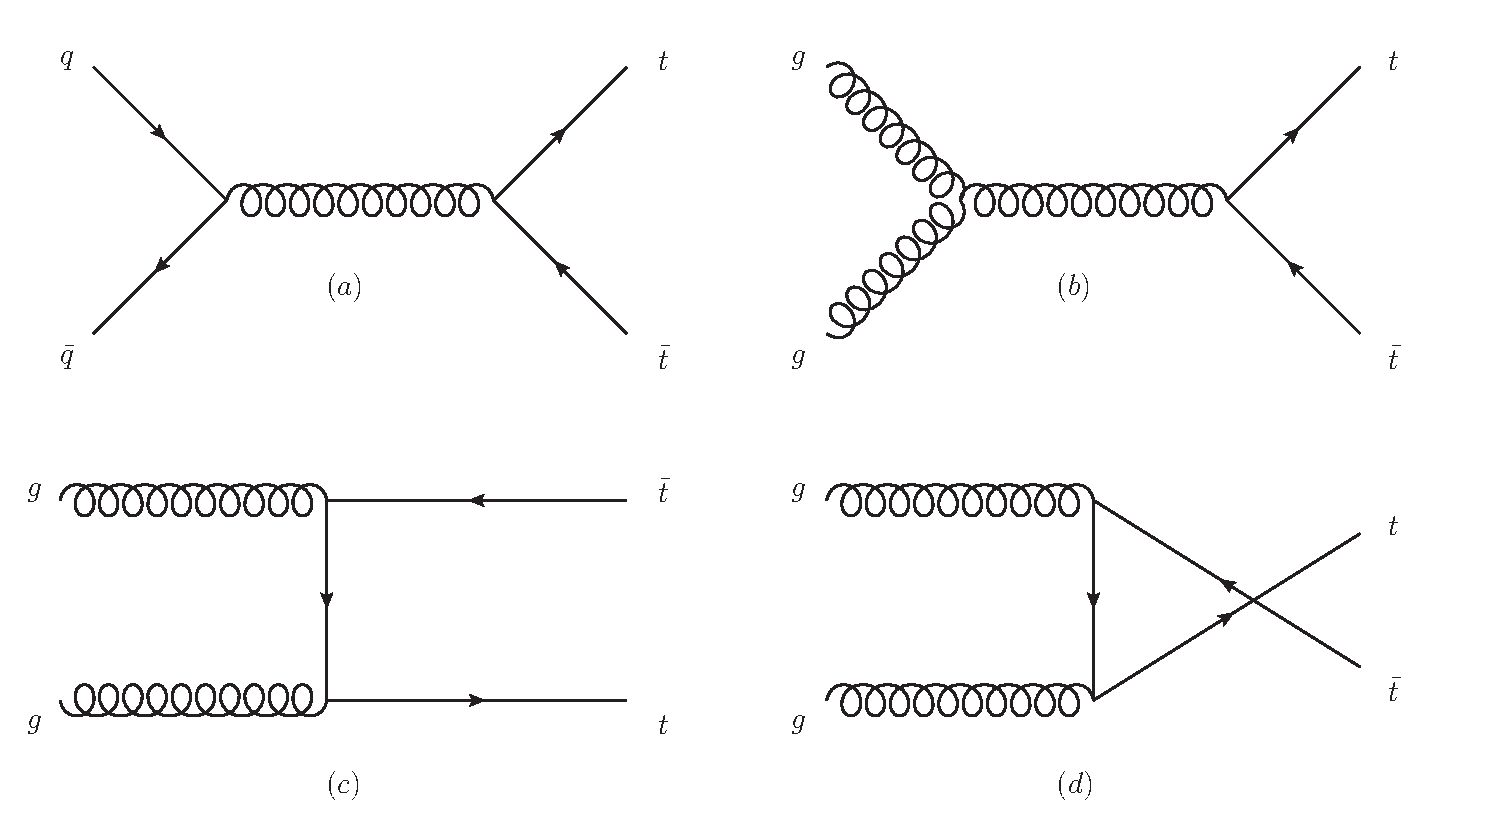
\includegraphics[width=0.9\textwidth]{Chapters/03_Theory/Images/ttbar_production}\hfill
     \caption[Feynman diagrams of leading order \ttbar production processes.]{Feynman diagrams of leading
     order \ttbar production processes. (a) depicts quark-antiquark annihilation, and (b, (c) and (d) depict
     gluon-gluon fusion in the s, t and u channels respectively.)}
     \label{fig:ttbar_production}
\end{figure}

\begin{figure}[hbtp]
   \centering
     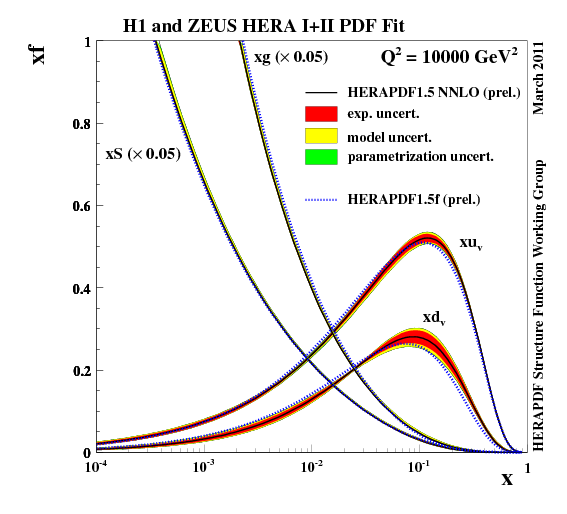
\includegraphics[width=0.7\textwidth]{Chapters/03_Theory/Images/proton_pdfs}
     \hfill
     \caption[Proton parton distribution functions at $Q^{2}=10\GeV^{2}$.]{Parton Distribution Functions
     (PDFs) from HERA as a function of proton momentum fraction for
     $Q^{2}=10\GeV^{2}$~\cite{Placakyte:2011az}}
     \label{fig:proton_parton_pdfs}
\end{figure}

At $\sqrt{s}=7\TeV$, gluon-gluon fusion accounts for approximately 80~\% of the total \ttbar production,
increasing to approximately 90~\% at $\sqrt{s}=14\TeV$ \cite{Agashe:2014kda}.
% A \ttbar production cross section of has been measured at $\sqrt{s}=7\TeV$ and at $\sqrt{s}=8\TeV$.

\begin{figure}[hbtp]
   \centering
     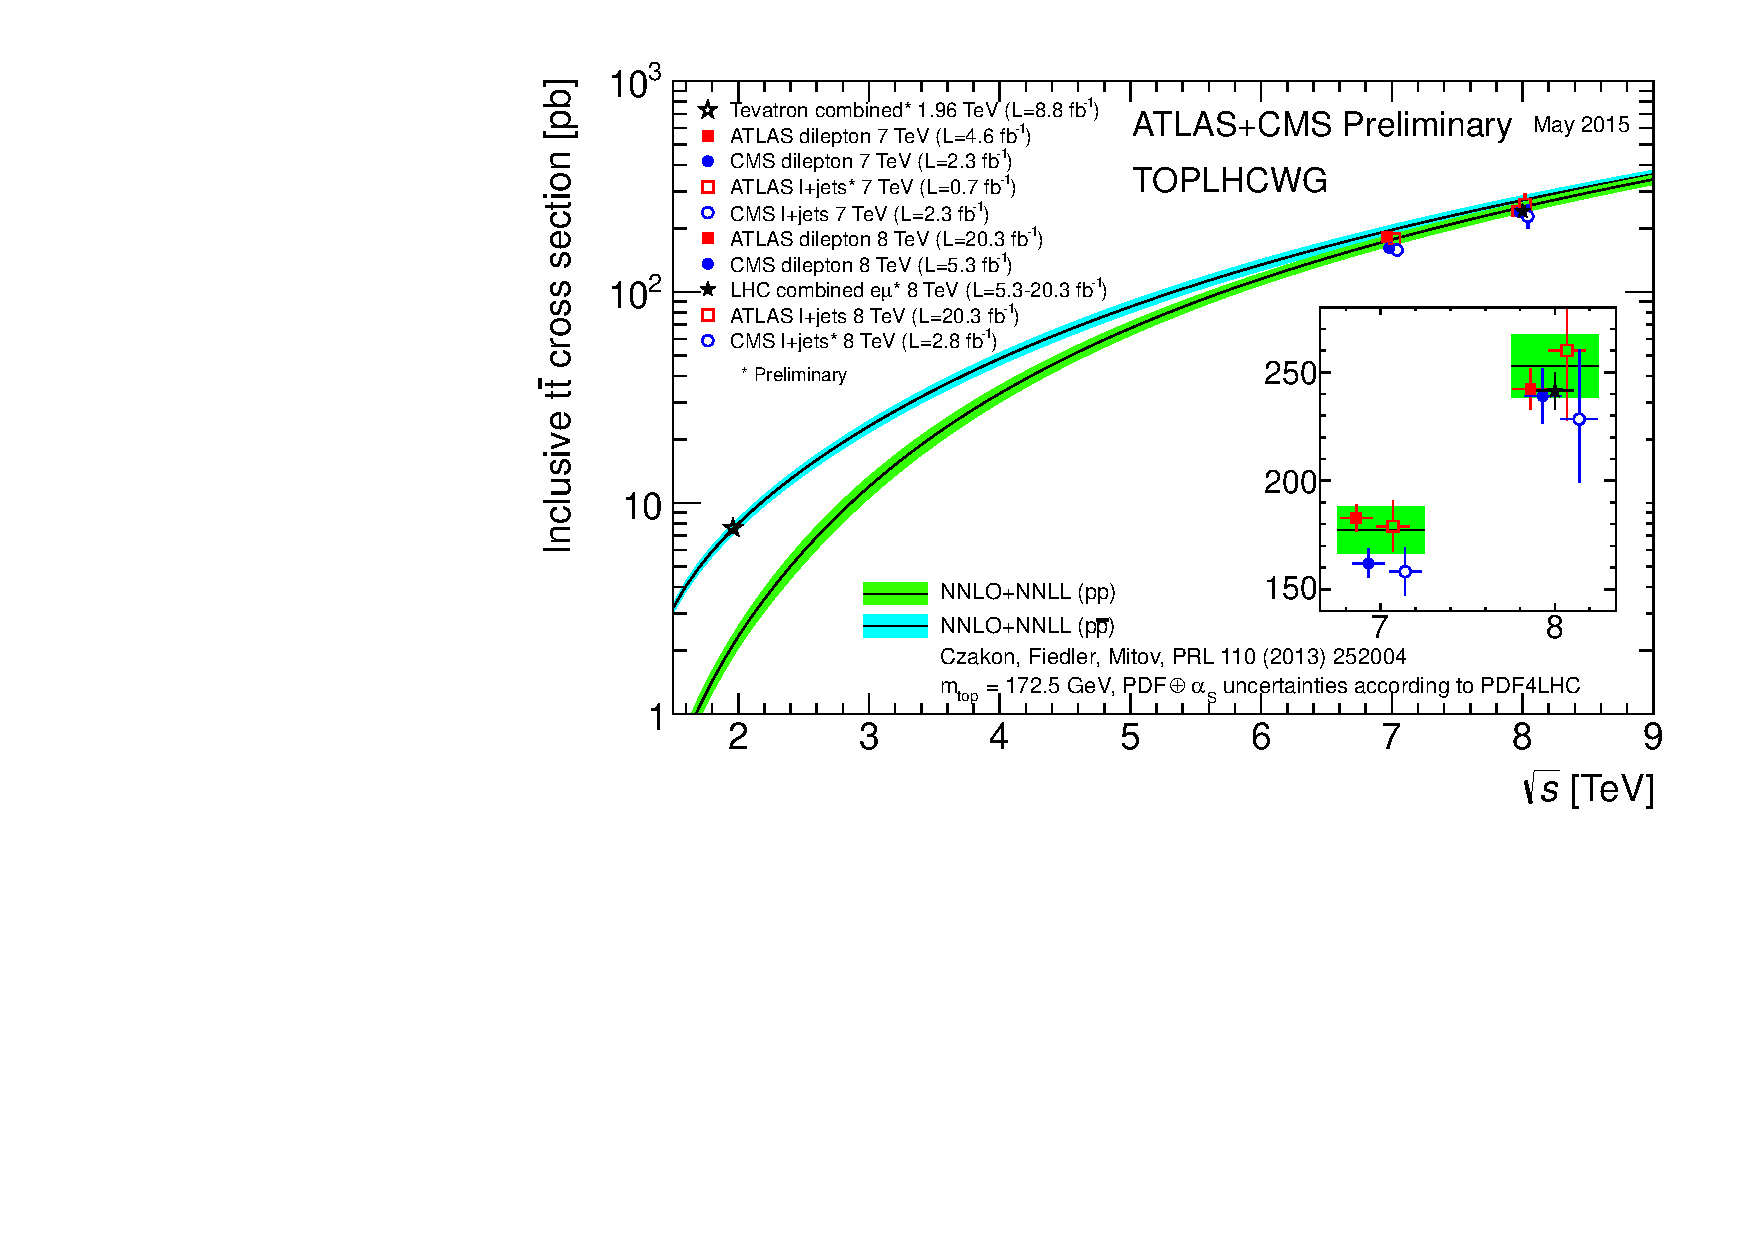
\includegraphics[width=0.8\textwidth]{Chapters/03_Theory/Images/toplhcwg_ttxsec_sqrts_may2015}\hfill
     \caption[\ttbar production cross sections at 1.96\TeV at CDF and D{\O} at the TeVatron and at 7\TeV and
     8\TeV at CMS and ATLAS at the LHC.]{\ttbar production cross sections at 1.96\TeV at CDF and D{\O} at the
     TeVatron and at 7\TeV and 8\TeV at CMS and ATLAS at the LHC~\cite{TOPLHC_WG}}
     \label{fig:ttbar_cross_sections}
\end{figure}

Top quarks decay almost 100~\% of the time to a \W boson and a \cPqb flavour jet. The \W boson then decays
either hadronically (into two jets) or leptonically (lepton + neutrino). Top pair events are characterised by the
decay of the \W bosons:
\begin{itemize}
  \item Leptonic: $\ttbar \rightarrow \W^{+} \cPqb \W^{-} \cPaqb \rightarrow l \nu_{l}\cPqb
  l' \bar{\nu_{l'}} \cPaqb$.
  Both \W bosons decay to a lepton and a neutrino. The event would consist of 2 jets, 2 leptons and 2
  neutrinos (which would show up as missing transverse energy (\met) in the event). (10.5~\%)
  \item Hadronic: $\ttbar \rightarrow \W^{+} \cPqb \W^{-} \cPaqb \rightarrow \cPq \cPaq \cPqb \cPq \cPaq
  \cPaqb$. Both \W bosons decay to two jets. The event would consist of 6 jets. (45.7~\%)
  \item Semi-Leptonic: $\ttbar \rightarrow \W^{+} \cPqb \W^{-} \cPaqb \rightarrow \cPq \cPaq \cPqb l \nu_{l}
  \cPaqb$. One \W boson decays to a lepton and a neutrino, the other decays to two jets. The event would
  consist of 4 jets, 1 lepton and 1 neutrino. This decay is shown in Figure~\ref{fig:semileptonic_decay}.
  (43.8~\%)
\end{itemize}

\begin{figure}[hbtp]
   \centering
     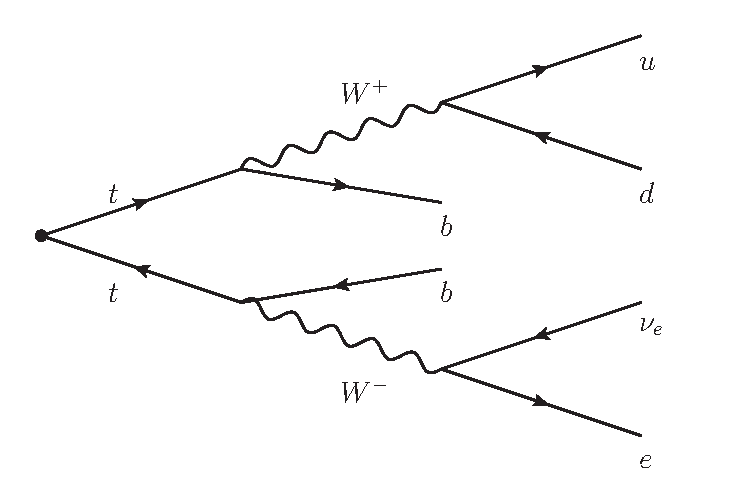
\includegraphics[width=0.7\textwidth]{Chapters/03_Theory/Images/semileptonic_decay}\hfill
     \caption[Feynman diagram of the electron+jets semi-leptonic \ttbar decay channel.]{Feynman diagram of the
     electron+jets semi-leptonic \ttbar decay channel.}
     \label{fig:semileptonic_decay}
\end{figure}

The branching ratios for each decay mode are quoted in brackets \cite{Agashe:2014kda}, and are represented
graphically in Figure~\ref{fig:ttbar_branching_ratios}. The numbers of jets in the final state of each channel
could be higher than the numbers quoted above as a result of higher order processes such as initial state
radiation (radiation from the gluons before the \ttbar production) or final state radiation. The hadronic
decay channel, with multiple jets and no leptons in the final state, is difficult to distinguish from the QCD
multijet, W+jets and Z+jets backgrounds. Conversely, the leptonic channel has a very clean signature with two
leptons, however the low branching ratio would limit the available statistics. The semi-leptonic channel, with
one lepton and four jets provides a good balance between statistics and event identification. The lepton can
be any of an electron, muon or $\tau$, but $\tau$s are not included in semi-leptonic \tquark analyses in
general as they are more difficult to identify (see Section~\ref{ss:experimental_uncertainties}).

\begin{figure}[hbtp]
   \centering
     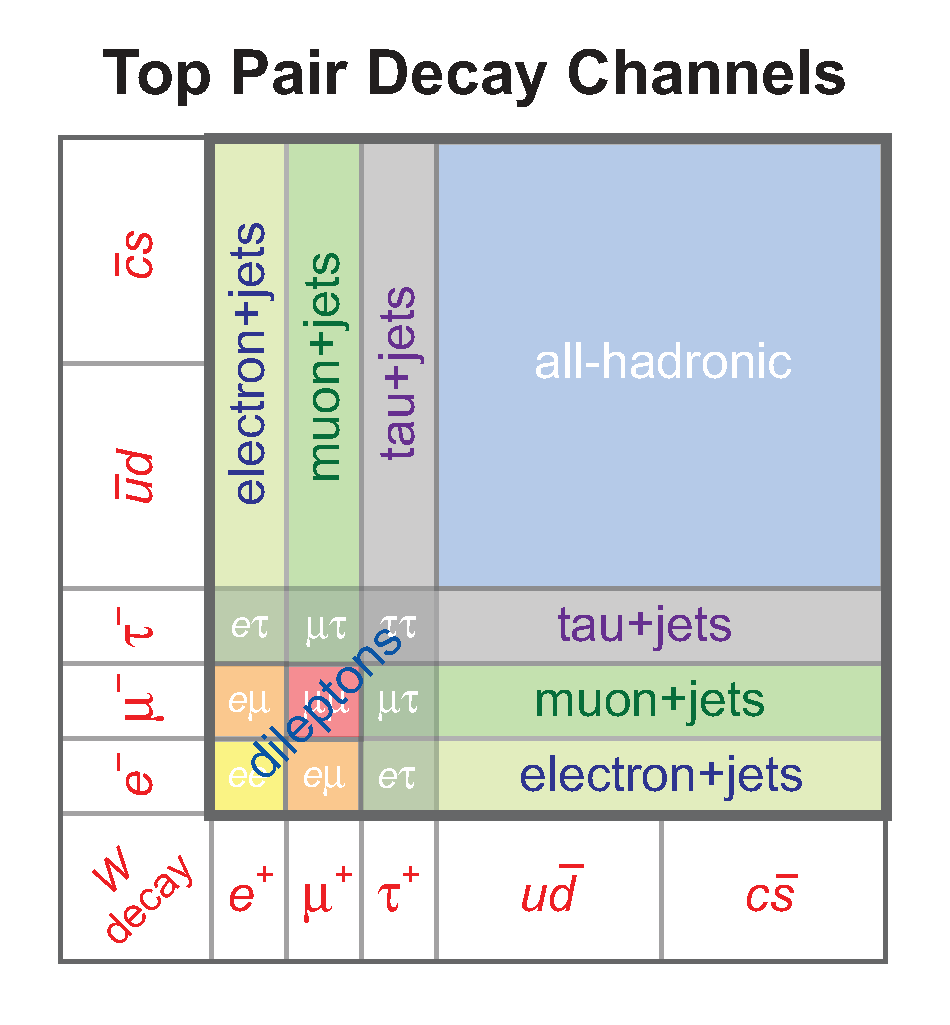
\includegraphics[width=0.5\textwidth]{Chapters/03_Theory/Images/top_pair_decay_channels}\hfill
     \caption[Relative branching ratios of the \ttbar system]{Relative branching ratios of the \ttbar system}
     \label{fig:ttbar_branching_ratios}
\end{figure}

The signal channel for the analysis described in this work is semi-leptonic \ttbar decay, also referred to as
the lepton+jets channel, where the lepton is either an electron or a muon. These channels have a branching
ratio of apprimxately 14.2~\% and 14.4~\% respectively \cite{Agashe:2014kda}.

\subsection{Single Top background}
\label{ss:single_top}
Single top production is one of the backgrounds considered in this analysis, and can occur via the electroweak
interaction in one of three channels: s-channel or t-channel which involve the exchange of a virtual \W boson,
or tW-channel which involves the associated production of a \W boson and a top quark. Although semi-leptonic
\ttbar decays have more jets in the final state than these single top production modes, initial state
radiation and final state radiation, where low energy gluons and quarks are produced before and after the
interaction that produces the single \tquark, can increase the numbers of jets in single top events. This can
lead to such events having a similar signature to \ttbar events, and providing a non-negligble background.

\subsection{W/Z+jets background}
\label{ss:w_z_plus_jets}
\WpJets production presents a significant background to semi-leptonic \ttbar analyses. This background
consists of events in which a real \W boson is produced together with additional jets. Events in which these
\W bosons decay leptonically can provide a similar event signature after reconstruction to that of a
semi-leptonic \ttbar decay. In general, these processes can be removed from the signal selection because the
final decay products in \WpJets events typically have lower energies than those from semi-leptonic \ttbar
decays, since the top quark has a high mass. Another characteristic of \WpJets events is that the jets are
more likely to be light quark jets and therefore less likely to be \bjets than in \ttbar events. Thus, \WpJets
events can be separated from the \ttbar signal by using jet multiplicity, jet \pt and \bjet multiplicity.

Similarly, \ZpJets events can mimic \ttbar events where the leptonic decay of a \Z boson to a lepton and an
anti-lepton takes place. This background can be distinguished from semi-leptonic \ttbar decays by
vetoing on a second lepton and imposing jet multiplicity requirements. Misidentification and misreconstruction
of these leptons as jets, however, can result in such events mimicking \ttbar events and passing the signal
selection, although this contamination is small.

\subsection{QCD background}
\label{ss:qcd}
The multijet background from QCD events presents a significant obstacle in many measurements at LHC, including
this semi-leptonic \ttbar analysis. Gluon-gluon fusion and quark-antiquark annihilation in proton-proton
collisions can produce energetic jets. Although these processes have only two jets in their final state,
higher order processes, including initial state radiation and final state radiation, can also produce
additional jets, leading to potential mimicking of the semi-leptonic \ttbar signal. The leptons required for
this to happen can come from jets which are misreconstructed and misidentified as leptons, or real leptons in
heavy flavour (\cPqb and \cPqc) jets. Unfortunately the cross section of these processes is several orders of
magnitude larger than the signal cross section. Although the lepton (either fake or real) is rarely one that
passes selection, the much higher QCD cross section means that its contribution as a background is
significant.
% TODO: READ LUKE'S THESIS FOR WAYS IN WHICH JETS CAN FAKE AN ELECTRON OR A MUON

In the muon+jets channel, only highly energetic jets ($\pt>500\GeV$) are capable of ``punching through'' from
the calorimeters to leave tracks in the muon chambers. Such events can be removed by isolation requirements
(since they deposit significant amounts of energy in the calorimeters). Events with real electrons and muons
from heavy quark jets can be identified by the track quality requirements in the selection since they would
not begin from the primary vertex and so would have a distinct track signature compared to prompt leptons.

On the other hand, the electron channel poses a more problematic QCD background, due mainly to the conversion
of photons, whether produced at the interaction point or through subsequent decays and radiation, into
electrons and positrons. The identification and removal of such events is described in
Section~\ref{ss:electron_reconstruction}. However, the large uncertainty in the cross sections of QCD events,
large contamination from higher order processes with additional jets in the signal region of this analysis and
the difficulty in modelling such contributions, lead to incorrect event kinematics and significant
disagreements in the QCD background distributions in data and in simulation. Therefore, the QCD background is
modelled using a data driven method, described in Section~\ref{ss:background_selection}, and then normalised
to the number of events passing the signal selection in simulation.

\section{Monte Carlo Simulation}
\label{s:monte_carlo_simulation}

Monte Carlo event simulation is used to simulate the aforementioned signal and background processes, and to
compare the theoretical knowledge of the SM incorporated therein with real data. Differences
between simulation and data would then indicate the presence of new physics processes which are not present in
the theoretical assumptions made in the SM, or perhaps that the simulation process is sub-optimal.
Different event generators exist, and samples produced by the \MADGRAPH, \PYTHIA, \POWHEG and \HERWIG
generators are used in this analysis.

Different generators have characteristics which optimise them for different aspects of the production chain:
the initial hard process scattering of the partons in the hadrons (protons), decay showers of the resulting
partons, subsequent decays of resulting hadrons and hadronisation of resulting partons, and the underlying
event (the parton showers produced from soft scattering between the remaining contents of the colliding
protons). 

\subsection{MadGraph}
\label{ss:madgraph}
\MADGRAPH \cite{madgraph5}, a matrix element generator, works by taking into account next-to-leading-order
Feynman diagrams for a given process and subsequently calculating the matrix elements for these diagrams over
all phase space. The Parton Distribution Functions are used to generate the incoming partons.
The cross section of the process and various subprocesses and the structure and contents of the event (such as
the partons present and their kinematics) are thus produced. %Also spin correlations. Also tau lepton decays
Proton fragmentation and subsequent hadronisation are simulated using the \PYTHIA generator, as explained in
Section~\ref{ss:pythia}.

The parton showers are then matched with the matrix element partons via the MLM method~\cite{mlm}. This
method ensures that parton showers with a highly energetic jet are not double counted. Matching is carried out
between parton showers in the hadronisation and the partons from the matrix element calculations. The matching
is carried out by satisfying distance requirements in $\eta$ and $\phi$ between the parton and parton shower.
Only if the parton has a transverse energy above a certain threshold, is it considered for this matching, and
if an event contains either too few or too many matching jets, it is discarded. The matching threshold is
process dependent as follows:

\onehalfspacing
\begin{itemize}
  \item \ttbar: 20\GeV
  \item \WpJets: 10\GeV
  \item \ZpJets: 10\GeV
\end{itemize}
\doublespacing

\subsection{MCatNLO}
\label{ss:mcatnlo}
The \MCATNLO \cite{mcatnlo_Frixione1, mcatnlo_Frixione2} generator is a next-to-leading-order generator. These
aditional corrections provide more accurate simulations of physics processes in comparison to leading-order
generators by including additional partons from the initial hard process in the final state of the event.

\subsection{PYTHIA}
\label{ss:pythia}
\PYTHIA \cite{pythia8} then simulates the proton fragmentation, the subsequent hadronisation of the
resulting quarks and gluons resulting from the hard interaction and the underlying event. \PYTHIA is
considered to be particuarly good at multi-particle simulation, modelling fragmentation and hadronisation, and
matching parton showers. Therefore, \PYTHIA carries out these steps after the initial partons are provided
by other generators in most simulated samples, if it is not already used for the whole production chain (as is
common in QCD multijet simulations).

\subsection{POWHEG}
\label{ss:powheg}
One problem with the \MCATNLO generator is that some events are given negative weights when matching
the next-to-leading-order QCD multijet calculations to parton showers.  The Positive Weight Hardest Emission
Generator, \POWHEG \cite{powheg_Frixione, powheg_Nason, powheg_Alioli}, is another next-to-leading-order
generator which generates the hardest processes in the event first, which avoids double counting of
softer radiation produced later in the chain, which is the cause of negative event weights.

%\subsection{HERWIG}
%\label{ss:herwig}
%\HERWIG \cite{herwig}
%TODO:HERWIG

\section{Theoretical Systematics}
\label{s:Theoretical Systematics}
\subsection{Factorisation \& Matching Threshold}
\label{ss:factorisation_and_matching_threshold}
The models used in generators use an essentially arbitrary choice for the threshold transverse energy above
which matrix-element partons are matched to parton showers. To account for the systematic uncertainties as a result
of this threshold, simulated samples in which the threshold is increased and decreased by a factor of 2 (see
Table~\ref{tab:matching_uncertainty_thresholds}) are used to estimate the affect of this uncertainty on this
analysis. Similarly, the factorisation scale at which $\alpha_{S}$ is varied up and down from the nominal
value of $Q^{2} = m^{2} + \Sigma p_{T}^{2}$ by a factor of 2 (see Table~\ref{tab:matching_uncertainty_thresholds}) to
produce simulation samples to evaluate the systematic uncertainty resulting from this. The uncertainty
resulting from these variations are evaluated in both \ttbar and \W/\ZpJets processes.

\begin{table}[hbth]
\centering
\resizebox{\columnwidth}{!} {
\begin{tabular}{|l|ccc|ccc|}
\hline
 & \multicolumn{3}{c}{Matching Threshold} & \multicolumn{3}{c}{Factorisation Scale} \\
Process & nominal / \GeV & + variation / \GeV & - variation / \GeV & nominal / \GeV & + variation / \GeV &  -
variation \\
\hline
\ttbar & 20 & 40 & 10 & $Q^{2} = m_{T}^{2} + \Sigma p_{T}^{2}$ & $(2Q)^{2}$ & $(0.5Q)^{2}$ \\
\WpJets & 10 & 20 & 5 & $Q^{2} = m_{W}^{2} + \Sigma p_{T}^{2}$ & $(2Q)^{2}$ & $(0.5Q)^{2}$ \\
\ZpJets & 10 & 20 & 5 & $Q^{2} = m_{Z}^{2} + \Sigma p_{T}^{2}$ & $(2Q)^{2}$ & $(0.5Q)^{2}$ \\
\hline
\end{tabular}
}
\caption{Threshold transverse energy for matching systematic uncertainty}
\label{tab:matching_uncertainty_thresholds}
\end{table}

\subsection{Detector Simulation (GEANT)}
\label{ss:detector_simulation}
Following creation of the physics processes in proton-proton collisions, the simulated events are then put
through a detector simulation to evaluate the interaction of the detector with the products of collisions. The
Geometry and Tracking 4 (\GEANTfour) package~\cite{Agostinelli:2002hh,Allison:2006ve} is used for this
purpose, which simulates what happens to particles as they travel through the geometry of the detector,
including simulation of the detector components and materials and the interaction of particles with the
detector such as particle tracks and energy deposits.